\subsubsection{Task realization}
Pomodoro is a simple technique for work organisation, specifically on computer. The 
idea is about making short breaks after each work session, usualy 5 min after 25.
In this way brain relaxes, eyes relax, and you return to work with new forces

For implementing this on mobile platform, I chosen Android Studio. App will consist 
from just one activity, with countdown and a button. Button will be necessary for
starting work session, and countdown is for user. And that's it, keeping it simple.
\begin{figure}[H]
    \centering
    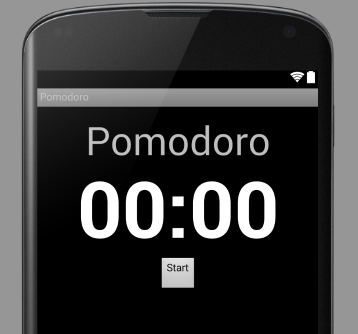
\includegraphics[width=0.7\textwidth]{screen1.png}
    \caption{Design}
    \label{fig:design}
\end{figure}

From GUI it is hard to edit layout, but from xml view there are more options. I used\\%texttt doesn't hyphenate
\texttt{android:gravity="center\_horizontal"} and found out 
\texttt{android:layout\_below="@+id/..."} (with corresponding (\emph{\_above, \_toLeftOf, \_toRightOf})
which are handy for arranging widgets on \emph{RelativeLayout}. Also here I added action
for button: \texttt{android:onClick="onStartPomodoro"}, and it will call the function with the same name:

\begin{verbatim}
    public void onStartPomodoro(View view){
        if(isPomodoroStarted) return; 
        final TextView countdown_display= (TextView)findViewById(R.id.countdown_display);
        final TextView app_status = (TextView)findViewById(R.id.appStatus);
        app_status.setText("Time to work");
        new CountDownTimer(pomodoro_time,1000){
            public void onTick(long millisUntilFinished){
                long minutes = millisUntilFinished/(60*1000);
                long seconds = (millisUntilFinished/1000) % 60;
                countdown_display.setText(String.format("%d:%02d",minutes, seconds));
            }
            public void onFinish() {
                notifyPomodoro();
                finishPomodoro();
            }
        }.start();
        isPomodoroStarted=true;
    }


\end{verbatim}

When countdown timer finishes, it will call 2 other functions, one for android notification, 
which will look like in Figure \ref{fig:notify}. This is necessary, because app is not intented
to be used permanently, the user just clicks button and may pause activity(switch to main menu or other
activity), but notification(with vibration) will be sent at respective time.
\begin{figure}[H]
    \centering
    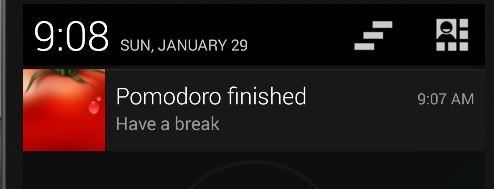
\includegraphics[width=0.9\textwidth]{screen2.png}
    \caption{Notificaiton}
    \label{fig:notify}
\end{figure}

For invoking notification:
\begin{verbatim}
    private void notifyPomodoro(){
        NotificationCompat.Builder mBuilder =
                new NotificationCompat.Builder(this)
                .setSmallIcon(R.drawable.tomato)
                .setContentTitle("Pomodoro finished")
                .setContentText("Have a break")
                .setAutoCancel(true)
                .setVibrate(new long[] {1000, 1000, 1000, 1000, 1000})
                .setLights(Color.RED, 3000, 3000);
        Intent resultIntent = new Intent(this, MainActivity.class);
        TaskStackBuilder stackBuilder = TaskStackBuilder.create(this);
        stackBuilder.addParentStack(MainActivity.class);
        stackBuilder.addNextIntent(resultIntent);
        PendingIntent resultPendingIntent =
                stackBuilder.getPendingIntent(
                        0,
                        PendingIntent.FLAG_UPDATE_CURRENT
                );
        mBuilder.setContentIntent(resultPendingIntent);
        NotificationManager mNotificationManager =
                (NotificationManager) getSystemService(Context.NOTIFICATION_SERVICE);
        mNotificationManager.notify(0,mBuilder.build());
    }
\end{verbatim}
Beside notification itself, I added action for opening app when clicking on notification. 
\texttt{setAutoCancel(true)} will configure notificaiton to close itself automatically if user
clicks it.

Pomodoro technique implies a longer rest periods after each 4 working sessions, that's why I
added a counter which will determine when halt should be small, and when to make it longer:
\begin{verbatim}
    private void finishPomodoro(){
        isPomodoroStarted = false;
        consecutive_pomodors++;
        int m = 1;//multiplier
        if(consecutive_pomodors==4) {
            m = 4;
            consecutive_pomodors = 0;
        }
        final TextView countdown_display= (TextView)findViewById(R.id.countdown_display);
        final TextView app_status = (TextView)findViewById(R.id.appStatus);
        app_status.setText("Relax time!");
        new CountDownTimer(m*rest_time,1000){
            public void onTick(long millisUntilFinished){
                long minutes = millisUntilFinished/(60*1000);
                long seconds = (millisUntilFinished/1000) % 60;
                countdown_display.setText(String.format("%d:%02d",minutes, seconds));
            }
            public void onFinish() {
                countdown_display.setText("00:00");
                app_status.setText("Time to work");
            }
        }.start();

    }
\end{verbatim}
When starting/finishing new working session, the text widget also changes.

For using images inside android app, I put the image itself in /res/drawable folder, and
also added an xml for telling sdk how to tag the image. All resources in android are 
accessed as members of \textbf{R} object. So image can be accessed as \texttt{R.drawable.}+\emph{image\_name}.
Widgets are accessed by \texttt{R.id}+\emph{\$\{android:id value from layout file\}}. 
